
	
% % % % % % % % % % % % % % % % % % % % % % % % % % % % % % % % % % % % % 	
% % % % % % % % % % % % % APENDICES % % % % % % % % % % % % % % % % % % %
% % % % % % % % % % % % % % % % % % % % % % % % % % % % % % % % % % % % % 	
\apendice %%%% TEXTOS A PARIR DESTE PONTO SERAO CONSIDERADOS APENDICES

\chapter{Demonstração de algo}
        \par Algo como apêndice.  
         \lipsum[2-10]

          
% % % % % % % % % % % % % % % % % % % % % % % % % % % % % % % % % % % % % % 	
% % % % % % % % % % % % % % % ANEXOS  % % % % % % % % % % % % % % % % % % % 
% % % % % % % % % % % % % % % % % % % % % % % % % % % % % % % % % % % % % % 	
        \anexo    %%%% TEXTOS A PARIR DESTE PONTO SERAO CONSIDERADOS ANEXOS
        
\chapter{Algo interessante que alguém fez}
         \par Algo como anexo.
         \lipsum[2-10]
                  
        \begin{grafico}[ht]
     	    \caption{\label{exepretex2}Orientações para a lombada do trabalho.}
	    \centering
	    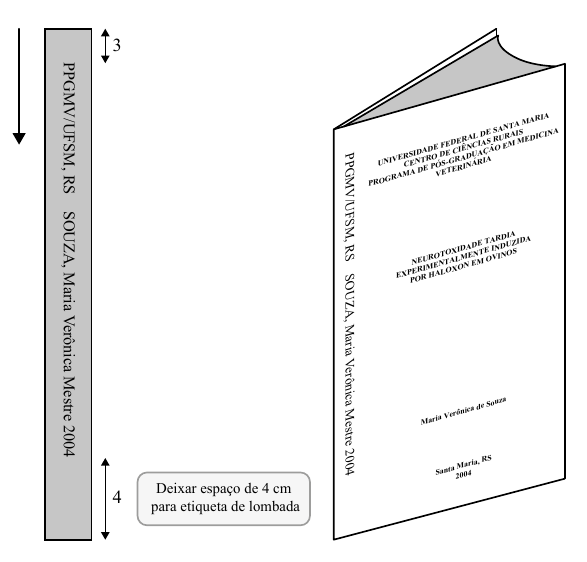
\includegraphics[width=0.6\textwidth]{figuras/lombada.png}
            \fonte{Adaptado de \citeonline{man:MDTUFSM2015}.}
         \end{grafico}         
         
         \lipsum[2-10]
